\chapter{Limitierungen \red[und Erweiterungen ]des Systems}
Ergänzend zu den zuvor aufgeführten Ergebnissen sollen in diesem Kapitel weitere Fehlereinflüsse und Limitierungen des \kps{s} diskutiert werden. Die vorgestellten Verfahren zur Selbstlokalisation und Darstellung visueller Zusatzinformationen für den Anwender sind allgemein anwendbar und hardwareunabhängig. Wie gezeigt wurde, konnte auf dem verwendeten System ein funktionierender Anwendungsablauf implementiert werden. Eine Erhöhung der Rechenleistung der verwendeten Komponenten würde sich demnach nicht auf das Funktionsprinzip des \kps{s} auswirken, könnte jedoch in verschiedenen Bereichen zu einer \red[Verbesserungen der Performance] führen. Durch den modularen Aufbau der Hard- und Software ist es jederzeit möglich einzelne Komponenten auszutauschen um die Robustheit oder Leistung des Gesamtsystems zu steigern.

\section{Lokalisation}
Eine möglichst präzise Annäherung der tatsächlichen Systempose ist Grundvoraussetzung für die Funktionalität des \kps{s}, da sie sich direkt auf die Projektionsgenauigkeit auswirkt.

Eine allgemeine Limitierung des Kinect Sensors ergibt sich durch das Verfahren zur Ermittlung der Tiefenwerte über die Projektion eines IR-Musters. Eine korrekte Erkennung des Musters kann nur gewährleistet werden, wenn die Beleuchtung der betrachteten Szene keinen \red[starken] IR Anteil aufweist. Insbesondere die Verwendung unter direktem Tageslichteinfall stellt deshalb ein Problem dar. Für den in dieser Arbeit behandelten Anwendungsfall der Lokalisation in geschlossenen Räumen kann dieser Aspekt jedoch vernachlässigt werden.

\subsection{Globale Lokalisation}
Die Auflösung des Kinect Sensors spielt besonders im Rahmen der globalen Lokalisation eine Rolle. Eine höhere Auflösung würde zu einem genaueren Abbild der Umgebung führen. Da vor der Lokalisation jedoch eine Filterung der Punktwolke erfolgt, so dass die Anzahl der betrachteten Punkte verringert wird, wäre ein Zugewinn an Präzision bei aktueller Konfiguration fraglich. Durch \red[Steigerung] der zur Verfügung stehenden Rechenleistung könnte jedoch die gefilterte Auflösung erhöht und die Lokalisationsgenauigkeit und -stabilität verbessert werden.\\

Eine Erhöhung der Rechenleistung könnte darüber hinaus Auch die für die globale Lokalisation benötigte Rechenzeit verringern beziehungsweise die Untersuchung einer größeren Anzahl von Partikeln ermöglichen.\\

\subsection{Visuelle Odometrie}
Das Tracking der Systempose basiert wie beschrieben auf dem Verfahren der visuellen Odometrie. Dazu werden kombinierte Merkmale aus den Aufnahmen der RGB-und IR-Kamera des Kinect Sensors extrahiert. Für eine robuste Bestimmung der Pose ist daher eine hinreichende Anzahl an Merkmalen zu detektieren. Ist die Umgebung nicht ausreichend ausgeleuchtet, können unter Umständen nicht genügend Merkmale bestimmt werden, woraus Fehler in der Lokalisation resultieren. 

\section{Projektion}

\subsection{Microvision ShowWX}
Der ShowWX Laser-Projektor verfügt über eine Helligkeit von etwa 15 Lumen. Dadurch kommt es bei Projektionen in stark ausgeleuchteten Umgebungen und bei größeren Entfernungen zur Projektionsfläche zu einem deutlichen Kontrastverlust.\red[ Bild?] Ein höherer Helligkeitswert würde somit den Anwendungsbereich erweitern. Diese Anforderung steht damit jedoch im Kontrast zu der Anforderung ausreichender Umgebungsausleuchtung für eine robuste visuelle Odometrie. Die Auswirkungen unterschiedlicher Beleuchtungsstärken der Umgebung zeigt \abb{fig.optlight}. Im Anwendungsfall gilt es somit, einen Kompromiss zu finden, welcher beiden Anforderungen gerecht wird.\\
%\red[In Kontrast setzen zu Anforderungen des Projektors -> optimale Helligkeit in der Mitte; Bilder für alle drei Anwendungsfälle aufnehmen?\\]

\begin{figure}[!ht]
	\begin{center}
		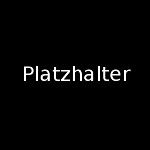
\includegraphics[scale=1.0]{spacer}
		\caption{Optimaler Helligkeitsbereich/Bilder die verdeutlichen wann visodom failt und wann Projektion zu undeutlich wird}
		\label{fig.optlight}
	\end{center}
	%\vspace*{-8mm}
\end{figure}

Anzumerken bleibt, dass eine Begrenzung der Leistung und damit auch der Helligkeit bei Laser-Projektoren durch die zulässige Laser-Klasse vorgegeben ist. Besonders im Bereich der tragbaren Projektoren sollte die Laser-Klasse 2\footnote{Klassifizierung nach EN 60825-1} nicht überschritten werden, da es sonst bei versehentlicher Betrachtung des Laserstrahls zu permanenter Schädigungen der Netzhaut kommen kann. Auch im Hinblick auf die \red[zuvor besprochene] Umgebungsausleuchtung sollte bei der Anwendung deshalb ein maximaler Abstand von etwa \red[TODO] zur Projektionsfläche nicht überschritten werden.\\

Eine weitere Möglichkeit eine deutlichere Darstellung der visuellen Zusatzinformationen zu erreichen, wäre neben einer Kontrast- beziehungsweise Helligkeitserhöhung auch eine Erhöhung der Auflösung der Projektion. Der ShowWX ist auf eine Auflösung von 480p begrenzt, wodurch es besonders bei feineren Strukturen trotz der Laser-Technologie zu unscharfen Abbildungen kommen kann.\\

\subsection{Raspberry Pi}
Für die über den Raspberry Pi realisierte Visualisierung eines \red[ROS-Topics] wurde die Totzeit bestimmt und mit der Ausführung des gleichen Programms auf einem Computer verglichen. Die wichtigsten Spezifikationen der Systeme sind zusammen mit den Ergebnissen der Untersuchung in \tab{totzeit} aufgeführt.

\begin{table}[ht]
\caption{Performance Vergleich zwischen Raspberry Pi und PC}
\begin{center}
\begin{tabular}{|l|c|c|}
\hline
\rowcolor{lightgray} & \multicolumn{1}{|c|}{\textbf{Raspberry Pi}} & \multicolumn{1}{|c|}{\textbf{Computer}}\\
\hline
Taktfrequenz & 700 Mhz & \\
\hline
Kerne & 1 & \\
\hline
Messungen & 20 & 20\\
\hline
Durchschnittliche Totzeit & & \\
\hline
\end{tabular}
\end{center}
\label{tab.totzeit}
\end{table}

Es zeigt sich, \red[TODO]\\
Das gekapselte Projektionsmodul bestehend aus dem Raspberry Pi und dem Microvision ShowWX ist damit \red[nicht geeignet/vergleichbar mit/...]\\
\red[Delay bzgl. raspberry -> Übertragung an anderen Rechner testen und Delay ebenfalls aufzeichnen\\]

\section{Interaktion}
Durch den minimalen aufgelösten Tiefenwert des Microsoft Kinect Sensors von \red[ABSTAND 0,8m?] ergibt sich eine Limitierung der aktuellen Systemkonfiguration bezüglich der Benutzerinteraktion. Um die Zeigerichtung robust erkennen zu können, ist es erforderlich, dass der Nutzer die Auswahl und Modifikation der Modellobjekte mit ausgestrecktem Arm durchführt. Eine kürzere minimale Distanz würde den Komfort bei der Eingabe deutlich erhöhen, da so die Interaktion bei verschiedenen Haltungen möglich wäre und der Benutzer bei längerer Interaktionsdauer entlastet werden würde.\\

Der minimale Tiefenwert definiert darüber hinaus auch den minimalen Abstand zur Projektionsfläche, da sowohl der globalen als auch der lokalen Lokalisation bei Unterschreiten dieses Abstands keine Umgebungsinformationen mehr zur Verfügung stehen. Es ergibt sich daraus zusammen mit dem definierten maximalen Projektionsabstand der in \abb{fig.optdist} dargestellte optimale Anwendungsabstand.\\
\red[Interaktionsbereich hier auch einzeichnen\\]
%\red[Empfehlung für Mindestabstand? Dann auch mit Kinect vergleichen und optimalen Betriebsbereich definieren; Bild, welches diesen darstellt?\\]

\begin{figure}[!ht]
	\begin{center}
		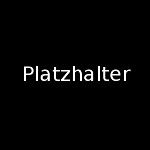
\includegraphics[scale=1.0]{spacer}
		\caption{Optimaler Abstand während der Verwendung des \kps{s}}
		\label{fig.optdist}
	\end{center}
	%\vspace*{-8mm}
\end{figure}


%\red[andere Struktur? Nicht Komponenten sondern Lokalisation, Projektion etc.?\\]

\red[TODO:\\
%Einleitender Absatz\\
%Limitierungen der Hardware\\
%Limitierungen der Lokalisation, global und lokal (Licht, features)\\
%Limitierungen des Projektors (Lichtstärke, Auflösung etc.)\\
Limitierungen in der Anwendung\\
Limitierungen in der Rechenleistung\\
]
%\section{Hardware}

%\section{Software}

%\section{Anwendung}